%*******************************************************************
% MAIN1
%*******************************************************************

\documentclass[a4paper,titlepage]{book}

%--------------------------------------------
% USEPACKAGES
%--------------------------------------------
\usepackage[utf8]{inputenc}
\usepackage[T1]{fontenc}
%!TEX encoding = UTF-8 Unicode
%\usefonttheme[onlymath]{serif}
\usepackage{listings}
\usepackage{lipsum}
\usepackage{caption}  
\usepackage[english]{babel}
\usepackage[swapnames]{frontespizio} 
\usepackage{textpos} %add the logo to the frametitle template using \addtobeamertemplate 
% https://texdoc.org/serve/textpos/0
\usepackage[hidelinks]{hyperref}
\urlstyle{same}
\usepackage{multicol}
\usepackage{graphics}
\usepackage{standalone}
\usepackage{multimedia}
\usepackage{media9}
\usepackage{graphicx}
\usepackage{empheq}
\usepackage{color}
\usepackage{siunitx}
\usepackage[many]{tcolorbox}
\usepackage{verbatim}
\usepackage{subfigure}
\usepackage{listings}
\usepackage{xcolor}
%\usepackage{palatino}
%\usepackage{euler}

%----------------------------
% ABSTRACT
%---------------------------
\usepackage{fancyhdr}


\begin{document}

%--------------------------------------------
% FRONTESPIZION
%--------------------------------------------
%https://tex.stackexchange.com/questions/161179/package-frontespizio
%https://ctan.mirror.garr.it/mirrors/ctan/macros/latex/contrib/frontespizio/frontespizio.pdf
% TO COMPILE:
% pdflatex [file].tex
% pdflatex [file-frn].tex
% pdflatex [file].tex
\begin{frontespizio}
    \begin{Preambolo*}
        %\usepackage{times}
        \usepackage{palatino}
        \newcommand{\VOF}{\textsc{vof}}
    \end{Preambolo*}
    \Istituzione{University of Pisa}
    \Logo[6.0cm]{figures/logo_unipi.jpg} 
    \Divisione{Department of Natural, Mathematical and Physical Sciences} 
    \Scuola{Master’s degree in Physics}
    \Titolo{Triggers fragmentation studies for FOOT experiment}
    \Relatore{Luca Galli} 
    \NRelatore{Thesis advisor}{} 
    \Correlatore{Bisogni Maria Giuseppina}
    \NCorrelatore{Research supervisor}{Research supervisors} 
    \NCandidato{Candidate}
    \Candidato{Lorenzo Marini} 
    \Piede{Academic Year 2021–2022}
\end{frontespizio}

% pdflatex [file].tex
% pdflatex [file-frn].tex
% pdflatex [file].tex

    %--------------------------------------------
    % DEDICA
    %--------------------------------------------
    %\begin{flushright}
Dedicato a qualcuno...
\end{flushright}

    %--------------------------------------------
    % ABSTRACT
    %--------------------------------------------
    \newenvironment{abstract}%
    {\cleardoublepage\thispagestyle{empty}\null\vfill\begin{center}%
    \bfseries\abstractname\end{center}}%
    {\vfill\null}
        \begin{abstract}
        This is the abstract.
        \end{abstract}




    %--------------------------------------------
    % INDICI
    %--------------------------------------------
    \tableofcontents
    \listoffigures
    \listoftables


    %--------------------------------------------
    % CAP 1
    %--------------------------------------------
    \chapter{Capitolo 1}


Prova del capitolo 1.

\begin{equation}
    F = ma
\end{equation}


\begin{equation}
    F = ma
\end{equation}


\begin{equation}
    F = ma
\end{equation}


\begin{equation}
    F = ma
\end{equation}



\begin{figure}
    \centering
    \begin{subfigure}[b]{0.15\textwidth}
        \centering
        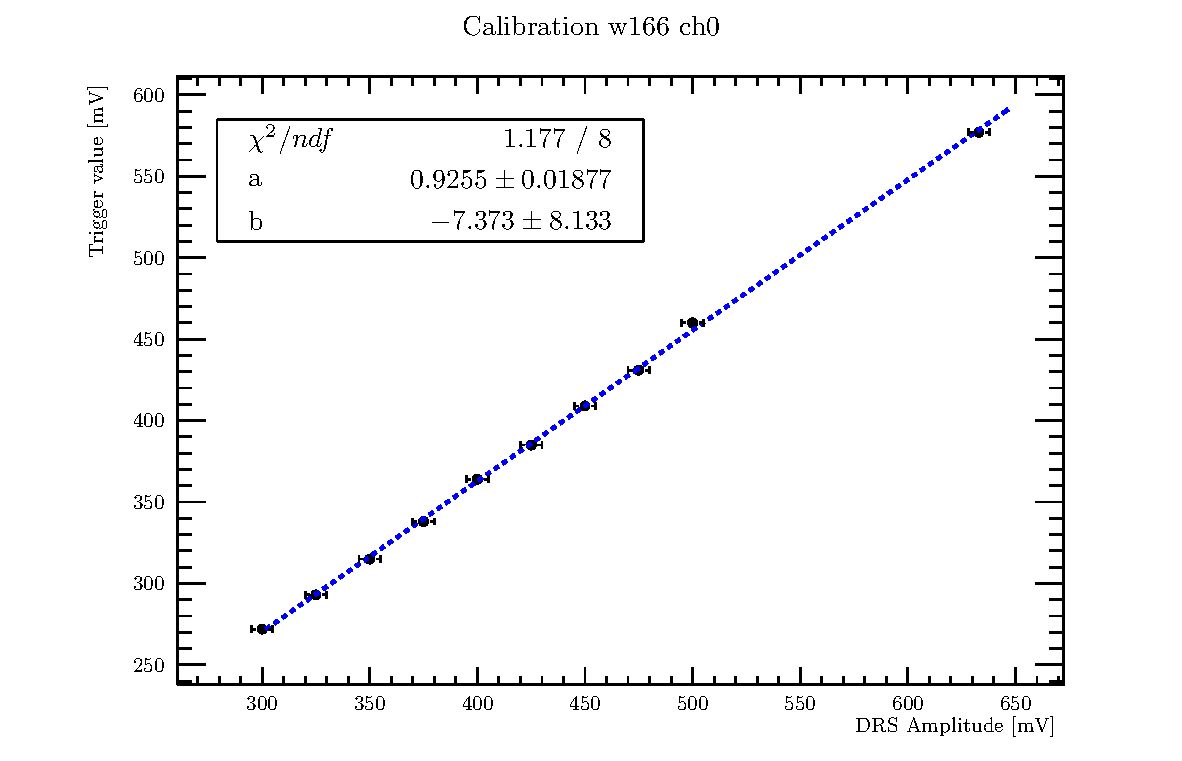
\includegraphics[width=\textwidth]{figures/ch0.pdf}
        \caption{$y=x$}
        \label{fig:y equals x}
    \end{subfigure}
    \hfill
    \begin{subfigure}[b]{0.15\textwidth}
        \centering
        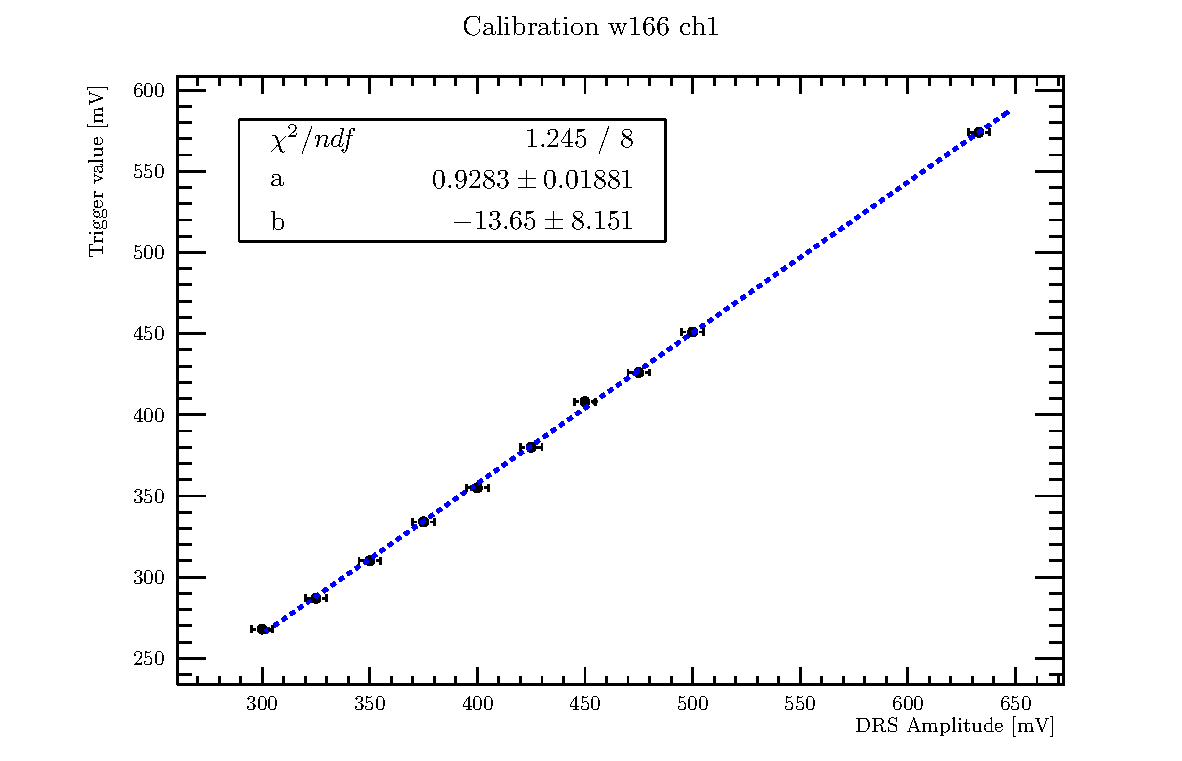
\includegraphics[width=\textwidth]{figures/ch1.pdf}
        \caption{$y=3sinx$}
        \label{fig:three sin x}
    \end{subfigure}
\end{figure}








        %--------------------------------------------
        \section{Prima sezione}


Qui ci scrivo qualcosa.
            \subsection{Sottosezione}

Scrivo qualcosa\cite{Pan}.
            \subsection{Sottosezione}

Scrivo qualcosa\cite{Pan}.
        \section{Prima sezione}


Qui ci scrivo qualcosa.
            \subsection{Sottosezione}

Scrivo qualcosa\cite{Pan}.
        \section{Prima sezione}


Qui ci scrivo qualcosa.
            \subsection{Sottosezione}

Scrivo qualcosa\cite{Pan}.
        %--------------------------------------------


    %--------------------------------------------
    % CAP 2
    %--------------------------------------------
    \chapter{Capitolo 2}

%==================================================================
				%SLIDE
%==================================================================
\begin{frame} [fragile]
\begin{equation*}
%\colorbox{yellow}{\text{Trigger value} =  a \times \text{DRS-Amplitude} + b}
\text{Trigger value} =  a \times \text{DRS-Amplitude} + b
\end{equation*}

\begin{center}
\begin{tabular}{ ccc } 
 \hline
\textbf{Channel} & a  [$\text{mV}^{-1}$]& b [mV] \\ 
 \hline
 \hline
00 & 0.9255 $\pm$ 0.01877 & -7.373 $\pm$ 8.133 \\ 
01 & 0.9283 $\pm$ 0.01881 & -13.65 $\pm$ 8.151 \\
02 & 0.925   $\pm$ 0.01876 & -9.959 $\pm$ 8.13 \\
03 & 0.9199 $\pm$ 0.01869 & -12.5   $\pm$ 8.1 \\
04 & 0.9169 $\pm$ 0.01865 & -9.624 $\pm$ 8.084 \\
05 & 0.9262 $\pm$ 0.01879 & -16.15 $\pm$ 8.142 \\
06 &    0.92  $\pm$ 0.0187   & -7.043 $\pm$ 8.102 \\
07 & 0.9217 $\pm$ 0.01872 & -12.57 $\pm$ 8.112 \\
08 & 0.8958 $\pm$ 0.02114 & -3.705 $\pm$ 8.988 \\
09 & 0.9109 $\pm$ 0.01803 & -13.49 $\pm$ 7.848 \\
10 & 0.9003 $\pm$ 0.01788 & -5.758 $\pm$ 7.782 \\
11 & 0.904 $\pm$ 0.01815   & -7.483 $\pm$ 7.884 \\
  \hline
  \hline
\end{tabular}
\end{center}
The parameters are different because the \textit{chips}, that are on the gain lines of all the channels, are different.
\end{frame}












%--------------------------------------------
% BIBLIOGRAPHY
%--------------------------------------------
\bibliographystyle{alpha}
\bibliography{biblio}
% pdflatex [filename].tex
% bibtex [filename]
% pdflatex [filename].tex
% pdflatex [filename].tex
% https://tex.stackexchange.com/questions/450863/using-bibtex-with-pdflatex

%--------------------------------------------
% END
%--------------------------------------------
\end{document}
